\section{Работа с файлами (Задание 8 вариант 1)}

\subsection{Условие задания}

Создать таблицу Student. В другой файл вывести студентов, у которых сдана сессия. (Вариант 1)

Приложение должно содержать следующие пункты:

\begin{enumerate}
    \item{Заголовок формы должен отражать суть задания.}

    \item{Все элементы формы должны быть внятно подписаны (кнопки подписаны, у тестового поля должно быть написано, для чего оно нужно и т.д.)}
    \item{Структура представляет собой таблицу DataGridView, в ячейках которой записаны данные разных типов.}
    \item {Предусмотреть кнопки:
        \begin{itemize}
            \item{считывание данных из файла и запись данных в таблицу (предполагается, что в файле данные корректные);}
            \item{возможность добавлять и удалять строки в таблице, соответственно, вводить данные вручную.}
            \item{запись в файл всех данных. Проверять корректность ввода данных: даты должны быть реальные, номер телефона состоять из цифр и, может быть, знак тире, оценки студентов --- от 2 до 5. Все остальное можно не проверять. Если есть срок пребывания, дата прибытия и дата отбытия, то срок пребывания должен быть равен разнице между датой отбытия и датой прибытия.}
            \item{запись в файл данных по определенному критерию. Критерий можно вводить вручную через TextBox или выбирать c помощью Radiobox и т. д. Запись в файл должна быть такой, чтобы этот файл можно было открыть в приложении.}
            \item{запись данных по определенному критерию в новую таблицу. При выборе другого критерия старая таблица должна удаляться.}
\end{itemize}
}
\item{При неправильном вводе каких"=либо данных таблица выбранных данных должна очищаться.}
    \item{В коде должны быть комментарии и отступы (код должен быть легко читаем).}
\end{enumerate}

\subsection{Вид формы в конструкторе}

Форма имеет вид (рис.\ref{fig:FormInConstruct8}):

\begin{figure}[!h]
    \centering
    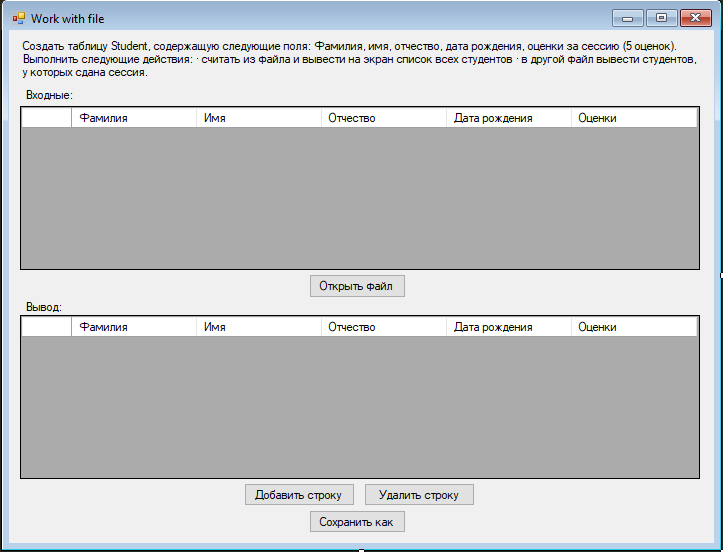
\includegraphics[width = 0.75\textwidth]{images/Task8/FormInConstructor.png}
    \caption{Вид формы в конструкторе}
    \label{fig:FormInConstruct8}
\end{figure}


\subsection{Таблица с описанием переименовнных элементов формы}

Все элементы формы были переименованы и их атрибыты изменены. Проведенные изменения представлены в таблице \ref{tab:label8}

\begin{longtable}[!h]{|l|l|l|}
    \caption{Значения атрибутов элементов в приложении <<Работа с файлами>>}
    \label{tab:label8}
    \hline
    \makecell{$\textbf{Описание элементов}$\\ $\textbf{формы}$}& \makecell{$\textbf{Список измененных}$\\ $\textbf{атрибутов}$}& \makecell{$\textbf{Новое значение}$\\ $\textbf{атрибута}$}\\ 
    \hline
    \makecell{Форма}& \makecell{Text}& \makecell{Work with file}\\ 
    \hline
    \makecell{Первая надпись (label)}& \makecell{Name}& \makecell{lblTask}\\ 
    \hline
    \makecell{Первая надпись (label)}& \makecell{Text}& \makecell{Создать таблицу\\ Student, содержащую\\ следующие поля:\\ Фамилия, имя,\\ отчество, дата\\ рождения, оценки\\ за сессию (5 оценок).\\ Выполнить следующие\\ действия: считать\\ из файла и вывести\\ на экран список\\ всех студентов;\\ в другой файл\\ вывести студентов,\\ у которых\\ сдана сессия.}\\ 
    \hline

    \makecell{Первая кнопка (button)}& \makecell{Name}& \makecell{btnReadFile}\\ 
    \hline
    \makecell{Первая кнопка (button)}& \makecell{Text}& \makecell{Открыть файл}\\ 
    \hline
    \makecell{Вторая кнопка (button)}& \makecell{Name}& \makecell{btnAddRow}\\ 
    \hline
    \makecell{Вторая кнопка (button)}& \makecell{Text}& \makecell{Добавить строку}\\ 
    \hline
    \makecell{Третья кнопка (button)}& \makecell{Name}& \makecell{btnRemoveRow}\\ 
    \hline
    \makecell{Третья кнопка (button)}& \makecell{Text}& \makecell{Удалить строку}\\ 
    \hline
    \makecell{Четвёртая кнопка (button)}& \makecell{Name}& \makecell{btnSaveInFile}\\ 
    \hline
    \makecell{Четвёртая кнопка (button)}& \makecell{Text}& \makecell{Сохранить как}\\ 
    \hline

    \makecell{Первая таблица\\ (dataGridView)}& \makecell{Name}& \makecell{dGrInput}\\ 
    \hline
    \makecell{Вторая таблица\\ (dataGridView)}& \makecell{Name}& \makecell{dGrOutput}\\ 
    \hline

    \makecell{Обработчик ошибок\\ (errorProvider)}& \makecell{Name}& \makecell{errPr}\\ 
    \hline

    \makecell{openFileDialog}& \makecell{Name}& \makecell{openFile}\\ 
    \hline

    \makecell{saveFileDialog}& \makecell{Name}& \makecell{saveFile}\\ 
    \hline
\end{longtable}

\subsection{Примеры работы}

При запуске приложения на экране появляется окно (рис.\ref{fig:StartForm8}).

\begin{figure}[!h]
    \centering
    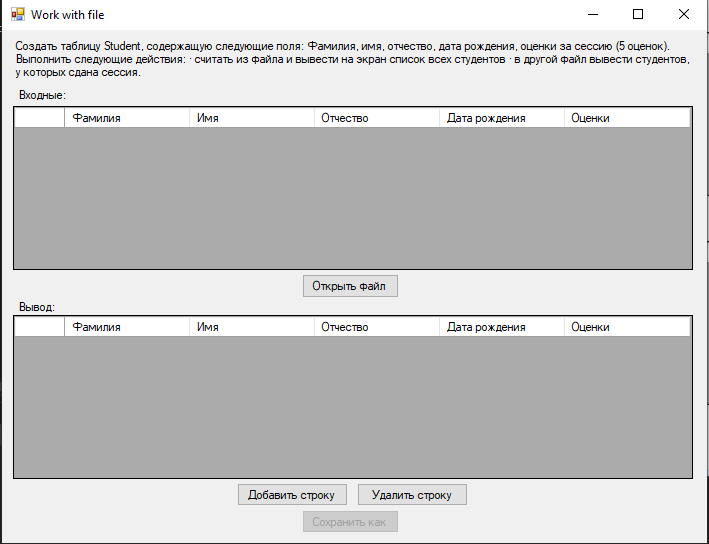
\includegraphics[width = 0.6\textwidth]{images/Task8/Start.png}
    \caption{Запуск приложения}
    \label{fig:StartForm8}
\end{figure}

При запуске с корректными данными, при нажатии на кнопку <<Открыть файл>> и выборе txt файла происходит (рис.\ref{fig:WorkForm8}):

\begin{figure}[!h]
    \centering
    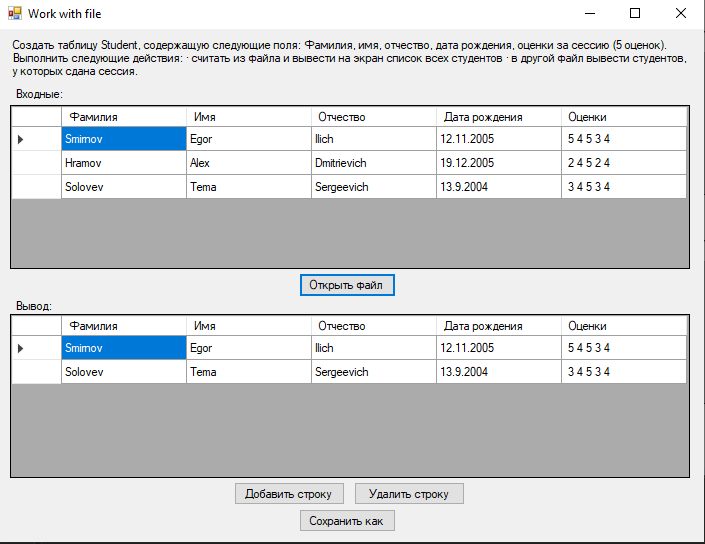
\includegraphics[width = 0.7\textwidth]{images/Task8/WorkOpenFile.png}
    \caption{Запуск с корректными данными}
    \label{fig:WorkForm8}
\end{figure}

При запуске с некорректными данными, при нажатии на кнопку <<Открыть файл>> и выборе txt файла происходит (рис.\ref{fig:BadInputNotIntForm8}):

\begin{figure}[!h]
    \centering
    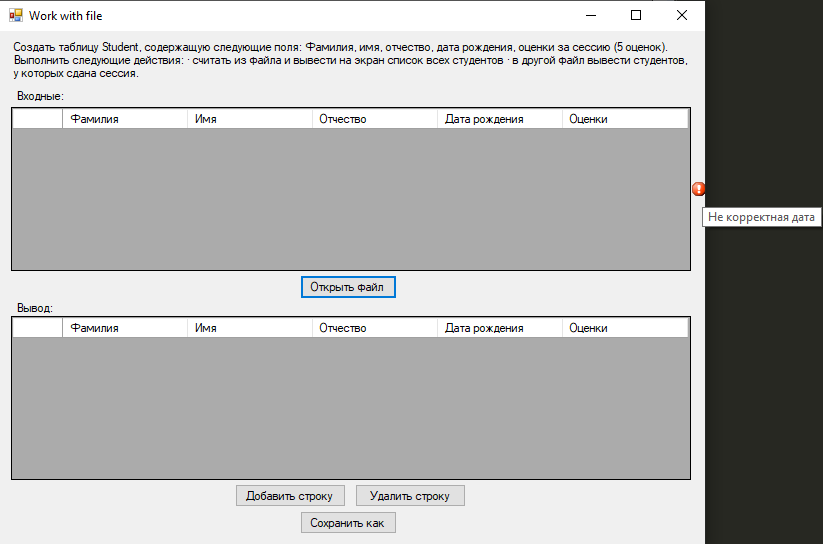
\includegraphics[width = 0.6\textwidth]{images/Task8/OpenFileBadData.png}
    \caption{Запуск с некорректными данными}
    \label{fig:BadInputNotIntForm8}
\end{figure}

\subsection{Примеры кода}

Функция сохранения в файл:

\begin{minted}{c++}
		// Сохранение файла
		private: System::Void btnSaveInFile_Click(System::Object^ sender, System::EventArgs^ e) {
			System::IO::Stream^ myStream;
			if (this->saveFile->ShowDialog() == System::Windows::Forms::DialogResult::OK)
				if ((myStream = saveFile->OpenFile()) != nullptr) {
					System::IO::StreamWriter^ sw =
						gcnew System::IO::StreamWriter(myStream,
							System::Text::Encoding::GetEncoding(1251)
						);
					try {
						for (int i = 0; i < this->dGrOutput->RowCount - 1; ++i) {
							sw->WriteLine(dGrOutputToString(i));
						}
						sw->Write(dGrOutputToString(this->dGrOutput->RowCount - 1));
					}
					catch (...) {
					}
					sw->Close();
				}
		}
\end{minted}

Другие фрагменты кода расположены в приложении \ref{app:task8}. Полный код программы приведен в приложении \ref{app:zip}
